\documentclass[12pt]{article}
\usepackage{tikz}
\usepackage{ifthen}
\usetikzlibrary{arrows}

% type, redundancy, required, lambda 
\newcommand{\modelgraphlabel}[4]{$#1$ \\ $r=#2$ \\ $\nu=#3$ \\ $\lambda=#4$}

\begin{document}
% Cloud Model 
% draw - outline, fill - color!alpha, align - allows for manual linebreak
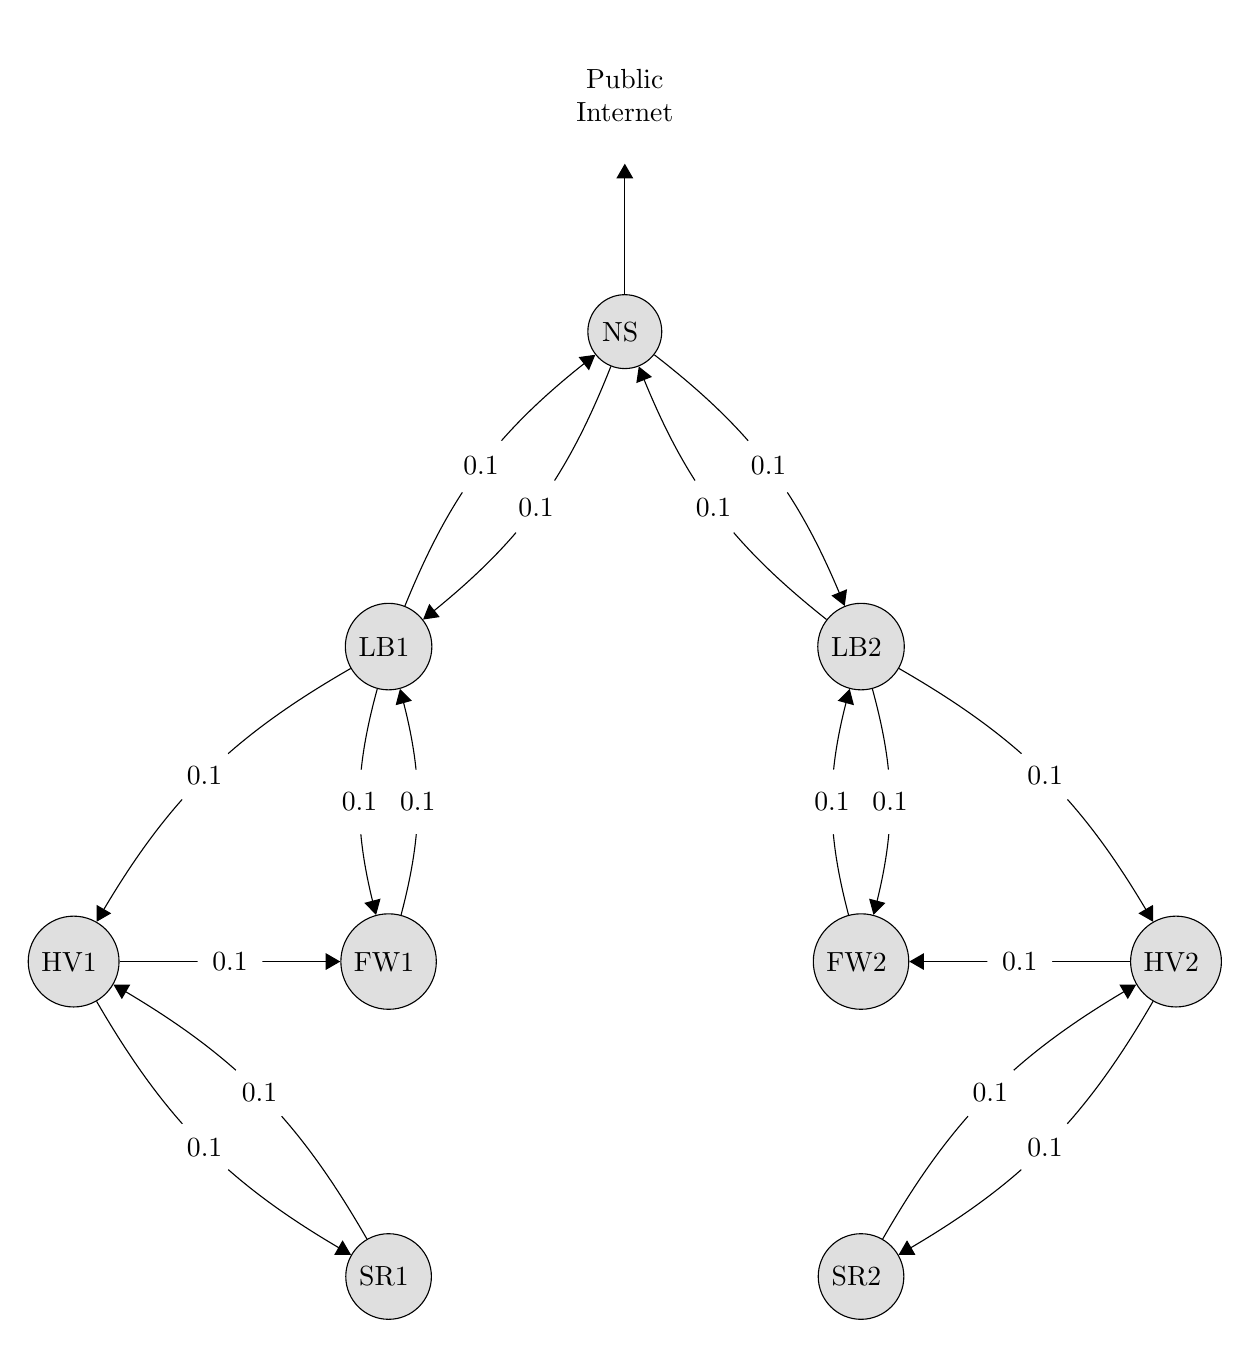
\begin{tikzpicture}[scale = 1, auto = center, every node/.style = {circle, draw = black, fill = gray!25}, bend angle = 90]

	\node (NS)  at ( 0, 16) [align = center] {\iffalse \modelgraphlabel{NS}  {2}{1} {0.01} \fi {NS}  };
	\node (LB1) at (-3, 12) [align = center] {\iffalse \modelgraphlabel{LB1} {2}{1} {0.01} \fi {LB1} };
	\node (LB2) at ( 3, 12) [align = center] {\iffalse \modelgraphlabel{LB2} {2}{1} {0.01} \fi {LB2} };
	\node (FW1) at (-3,  8) [align = center] {\iffalse \modelgraphlabel{FW1} {2}{1} {0.01} \fi {FW1} };  
	\node (FW2) at ( 3,  8) [align = center] {\iffalse \modelgraphlabel{FW2} {2}{1} {0.01} \fi {FW2} };
	\node (HV1) at (-7,  8) [align = center] {\iffalse \modelgraphlabel{HV1} {2}{1} {0.01} \fi {HV1} };
	\node (HV2) at ( 7,  8) [align = center] {\iffalse \modelgraphlabel{HV2} {2}{1} {0.01} \fi {HV2} };  
	\node (SR1) at (-3,  4) [align = center] {\iffalse \modelgraphlabel{SR1} {3}{2} {0.01} \fi {SR1} };
	\node (SR2) at ( 3,  4) [align = center] {\iffalse \modelgraphlabel{SR2} {3}{2} {0.01} \fi {SR2} };
	\node (PB)  at ( 0, 19) [align = center, fill=none, draw=none] {Public\\Internet};

    \foreach \from/\phy/\to in {NS/0.1/LB1, NS/0.1/LB2, LB1/0.1/NS, LB2/0.1/NS, 
    LB2/0.1/FW2, FW2/0.1/LB2, LB2/0.1/HV2, SR2/0.1/HV2, HV2/0.1/SR2}
    	\path (\from) edge [-triangle 60, bend left = 15] node[fill=white, draw=none] {\phy} (\to);
    \foreach \from/\phy/\to in {LB1/0.1/FW1, FW1/0.1/LB1, LB1/0.1/HV1, SR1/0.1/HV1, HV1/0.1/SR1}
    	\path (\from) edge [-triangle 60, bend right = 15] node[fill=white, draw=none] {\phy} (\to);
    \foreach \from/\phy/\to in {HV1/0.1/FW1,HV2/0.1/FW2}
    	\path (\from) edge [-triangle 60] node[fill=white, draw=none] {\phy} (\to);

    \path (NS) edge [-triangle 60] node[fill=none, draw=none] {} (PB);

\end{tikzpicture}

\newpage

We now consider a model representing a cloud computing architecture. NS represents a Network Switch; LB1, 2 represent two types of Load Balancers; FW 1, 2 represent two types of firewalls; HV 1, 2 represent two types hypervisors and SR 1, 2 represent two types of server racks. This organization of components specifically shows a firewall ``sandwich" as described in \cite{Salch:2004}. 

$r_NS$   

\bibliographystyle{plain}
\bibliography{cloud} 

\end{document}